\subsection{Validation}

\begin{frame}{Validation}
  \begin{itemize}
    \item \alert{Montrer que RenamableLogootSplit satisfait la cohérence forte à terme}
    \item \alert{Montrer que le mécanisme de renommage améliore les performances} de la séquence répliquée (mémoire, calculs, bande-passante)
  \end{itemize}
  \pause
  \begin{center}
    \alert{Conduite d'une évaluation expérimentale}
  \end{center}
\end{frame}

\begin{frame}[standout]
  \alert{Absence d'un jeu de données de sessions d'édition collaborative}

  \medskip
  \pause
  Mise en place de simulations pour générer un jeu de données
\end{frame}

\begin{frame}{Simulations - Architecture}
  \begin{figure}
    \centering
    \resizebox{0.5 \columnwidth}{!}{
      \begin{tikzpicture}
        \path
          +(90:10) node (a) {\includegraphics[page=5, trim=0cm 24cm 32cm 0cm, clip]{img/mute-figures.pdf}}
          +(-90:10) node (b) {\includegraphics[page=5, trim=0cm 24cm 32cm 0cm, clip]{img/mute-figures.pdf}}
          +(180:5) node (c) {\includegraphics[page=5, trim=0cm 24cm 32cm 0cm, clip]{img/mute-figures.pdf}}
          ++(0:10)
          +(90:10) node (d) {\includegraphics[page=5, trim=0cm 24cm 32cm 0cm, clip]{img/mute-figures.pdf}}
          +(-90:10) node (e) {\includegraphics[page=5, trim=0cm 24cm 32cm 0cm, clip]{img/mute-figures.pdf}}
          +(0:5) node (f) {\includegraphics[page=5, trim=0cm 24cm 32cm 0cm, clip]{img/mute-figures.pdf}};

        \draw[latex-latex, line width=1.5mm]
          (a) edge (b) (a) edge (c) (a) edge (d) (a) edge (e) (a) edge (f)
          (b) edge (c) (b) edge (d) (b) edge (e) (b) edge (f)
          (c) edge (d) (c) edge (e) (c) edge (f)
          (d) edge (e) (d) edge (f)
          (e) edge (f);
      \end{tikzpicture}
    }
  \end{figure}
  \begin{itemize}
    \item \alert{10 noeuds} éditent collaborativement un document
    \item Topologie \alert{réseau entièrement maillée}
    \item Ne considère \alert{pas de pannes ou de pertes de message}
  \end{itemize}
\end{frame}

\begin{frame}{Simulations - Modifications}
  \metroset{block=transparent}
  \begin{block}{Se décompose en 2 phases}
    \begin{enumerate}
      \item \alert{Génération du contenu} (80\% d'\ins, 20\% de \rmv)
      \item \alert{Édition} (50/50\%)
    \end{enumerate}
    Noeuds passent à la phase 2 quand leur copie locale atteint une taille donnée (15 pages - 60k caractères)
  \end{block}
  \pause
  \textbf{Nombre d'opérations : } 15k par noeud, 150k au total
\end{frame}

\begin{frame}{Simulations - Mécanisme de renommage}
  \metroset{block=transparent}
  Noeuds \alert{utilisent LogootSplit} (LS) ou \alert{RenamableLogootSplit} (RLS)
  \pause
  \begin{block}{Noeuds de renommage}
    \begin{itemize}
      \item 1 à 4 noeuds effectuent une \alert{opération \ren toutes les 30k opérations}
      \item Opérations \ren générées à un point donné sont \alert{concurrentes}
    \end{itemize}
  \end{block}
\end{frame}

\begin{frame}{Simulations - Sorties \& résultats}
  \metroset{block=transparent}
  \begin{itemize}
    \item \alert{Instantané de l'état} de chaque noeud à différents points de la simulation (10k opérations et état final)
    \item \alert{Journal des opérations} de chaque noeud
  \end{itemize}
  \pause

  \begin{block}{Conduite d'évaluations sur ces données\singlefootnote{Code des simulations et benchmarks : \url{https://github.com/coast-team/mute-bot-random}}}
    \begin{itemize}
      \item Validation de l'amélioration des performances de la séquence répliquée (mémoire, calculs, bande-passante)
    \end{itemize}
  \end{block}

\end{frame}
